\documentclass[11pt]{article}
\usepackage[notes]{la}
\lamodule{3}{2}{Properties of Determinants}
\laxdoc{2.2}
\laxdoc{2.3}
\laxdoc{3.1}

\begin{document}

\section{Properties of Determinants}

\begin{guide}
Cofactor expansion needs more than $n!$ multiplications (Example~\ref{3.1-ex:cost}), yet a triangular matrix has a determinant that we can read off (Theorem~\ref{3.1-thm:triangular}). Row reduction turns every square matrix into a triangular one in about $n^3$ steps. If we knew what each row operation does to the determinant, we could compute determinants by elimination. And what is the determinant for? We saw that it is zero for matrices with a zero row or column and for singular triangular matrices. Is $\det A\neq0$ really the same as ``$A$ is invertible'' for every square matrix? How does it behave under products?
\end{guide}

\textbf{By the end of this section you should be able to:}
\begin{itemize}
  \item state how replacement, interchange and scaling of a row change a determinant, and explain why;
  \item compute a determinant by row reduction, keeping track of interchanges and scalings, and compare the result with cofactor expansion;
  \item show that a matrix with two equal rows, or a row that is a multiple of another row, has determinant zero;
  \item state and use the theorem ``$A$ is invertible if and only if $\det A\neq0$'' as one more statement of the Invertible Matrix Theorem;
  \item use the product rule $\det AB=\det A\det B$, and its consequences for $\det A\T$, $\det A^{-1}$ and $\det A^k$, without computing the matrices involved;
  \item avoid the traps $\det(A+B)\neq\det A+\det B$ and $\det(rA)\neq r\det A$;
  \item use column operations, and interpret $|\det A|$ as the factor by which $A$ changes areas (in the plane) and volumes (in space).
\end{itemize}

% ---------------------------------------------------------------------
\subsection*{What a row operation does to the determinant}

In Section 3.1 (Pause and think~\ref{3.1-think:faster}) we tried the three elementary row operations on $\begin{bmatrix}1&2\\3&4\end{bmatrix}$, whose determinant is $-2$. Replacement ($R_2-3R_1$) gave $-2$ again, an interchange gave $+2$, and doubling a row gave $-4$. The next theorem says that this is no accident.

\begin{thm}{Row operations and the determinant}{rowops}
Let $A$ be a square matrix.
\begin{enumerate}
  \item[(a)] If a multiple of one row of $A$ is added to another row to produce a matrix $B$ (a \emph{replacement}), then $\det B=\det A$.
  \item[(b)] If two rows of $A$ are interchanged to produce $B$, then $\det B=-\det A$.
  \item[(c)] If one row of $A$ is multiplied by a number $k$ to produce $B$, then $\det B=k\det A$.
\end{enumerate}
\end{thm}

\begin{proof}
For $1\times1$ matrices only scaling is possible, and $\det[ka]=k\det[a]$. We prove the theorem for $n\times n$ matrices with $n\geq2$ by induction on $n$.

\emph{Size $2\times2$.} Let $A=\begin{bmatrix}a&b\\c&d\end{bmatrix}$. (a)~Adding $k$ times row $1$ to row $2$ gives $a(d+kb)-b(c+ka)=ad-bc$; adding $k$ times row $2$ to row $1$ gives $(a+kc)d-(b+kd)c=ad-bc$. (b)~Interchanging the rows gives $cb-da=-(ad-bc)$. (c)~Multiplying row $1$ by $k$ gives $kad-kbc=k(ad-bc)$, and multiplying row $2$ by $k$ gives $akd-bkc=k(ad-bc)$.

\emph{From size $n-1$ to size $n$, where $n\geq3$.} Assume the theorem for matrices of size $n-1$. The operation involves at most two rows of $A$. Since $n\geq3$, there is a row $i$ that it does not involve, so row $i$ of $B$ equals row $i$ of $A$: $b_{ij}=a_{ij}$ for every $j$. Delete row $i$ and column $j$ from both matrices. The matrix $B_{ij}$ arises from $A_{ij}$ by the \emph{same} operation (the rows involved are still present, with column $j$ removed). By the assumption, $\det B_{ij}=c\det A_{ij}$ where $c=1$ for a replacement, $c=-1$ for an interchange and $c=k$ for a scaling. Expanding along row $i$ (Theorem~\ref{3.1-thm:expansion}),
\[
\det B=\sum_{j=1}^{n}(-1)^{i+j}b_{ij}\det B_{ij}=c\sum_{j=1}^{n}(-1)^{i+j}a_{ij}\det A_{ij}=c\det A.
\]
\end{proof}

\begin{kc}{What do the operations do?}{effects}
Suppose a $3\times3$ matrix $A$ has $\det A=7$. Find the determinant of the matrix $B$ obtained from $A$ by (a)~replacing $R_2$ by $R_2+3R_1$; (b)~interchanging $R_1$ and $R_3$; (c)~multiplying $R_2$ by $5$; (d)~multiplying $R_3$ by $\tfrac17$ and then interchanging $R_1$ and $R_2$; (e)~multiplying \emph{every} row by $2$.
\end{kc}

\begin{thm}{Two rows that are proportional}{equalrows}
If two rows of a square matrix $A$ are equal, or if one row is a multiple of another row, then $\det A=0$.
\end{thm}

\begin{proof}
Suppose row $p$ is $c$ times row $q$ (with $c=1$ for equal rows). The replacement $R_p-cR_q$ produces a matrix with a row of zeros, which has determinant $0$ (Theorem~\ref{3.1-thm:zero}). By Theorem~\ref{thm:rowops}(a) the replacement did not change the determinant, so $\det A=0$.
\end{proof}

\begin{think}{A second proof by interchanging}{swap}
(a)~Suppose rows $p$ and $q$ of $A$ are equal. What happens to the matrix if you interchange them? What does Theorem~\ref{thm:rowops}(b) say about $\det A$ then? Conclude that $\det A=0$ without using a row of zeros. (b)~Does the same argument show that a matrix whose rows are merely proportional, say row $p$ equal to $3$ times row $q$, has determinant $0$? What extra step is needed? (c)~In Pause and think~\ref{3.1-think:signs} the alternating signs were forced by a matrix with two equal rows. Which part of the proof of Theorem~\ref{thm:rowops} is the same idea?
\end{think}

\begin{thm}{Elementary matrices}{elementary}
Let $E$ be an elementary matrix. Then $\det E=1$ if $E$ replaces a row, $\det E=-1$ if $E$ interchanges two rows, and $\det E=k$ if $E$ multiplies a row by $k$. For every square matrix $A$ of the same size,
\[
\det(EA)=(\det E)(\det A).
\]
\end{thm}

\begin{proof}
$E$ arises from the identity matrix by one row operation, and $\det I=1$ (Theorem~\ref{3.1-thm:triangular}). By Theorem~\ref{thm:rowops} its determinant is $1$, $-1$ or $k$. By Theorem~\ref{2.2-thm:elementary}, $EA$ is the matrix obtained from $A$ by the same row operation, so by Theorem~\ref{thm:rowops} again $\det(EA)$ is $1$, $-1$ or $k$ times $\det A$.
\end{proof}

% ---------------------------------------------------------------------
\subsection*{Computing a determinant by row reduction}

Elimination uses replacements and, when a pivot position holds a zero, interchanges. Neither needs a scaling. Reduce $A$ to an echelon form $U$ using only these two operations, and count the interchanges. A square echelon form is upper triangular, so $\det U$ is the product of its diagonal entries (Theorem~\ref{3.1-thm:triangular}), and the replacements did not change the determinant:
\[
\det A=(-1)^{r}\,u_{11}u_{22}\cdots u_{nn},\qquad r=\text{the number of interchanges.}
\]

\begin{proc}{Determinant by row reduction}{reduce}
\begin{enumerate}
  \item Reduce $A$ to an echelon form $U$ with replacements and interchanges. Write down the number $r$ of interchanges.
  \item If $U$ has a zero on its diagonal, $\det A=0$.
  \item Otherwise $\det A=(-1)^r\times$ (product of the diagonal entries of $U$).
  \item If you also multiplied rows by numbers $k_1,\dots,k_s$ (try to avoid this), then $\det A=(-1)^r\,u_{11}\cdots u_{nn}\big/(k_1\cdots k_s)$.
\end{enumerate}
\end{proc}

\begin{exmp}{Reduction with an interchange}{reduce}
Let $A=\begin{bmatrix}0&3&-2\\1&2&1\\2&1&3\end{bmatrix}$. The entry $a_{11}$ is zero, so interchange the first two rows:
\begin{align*}
\begin{bmatrix}0&3&-2\\1&2&1\\2&1&3\end{bmatrix}
&\rops{R_1\leftrightarrow R_2}
\begin{bmatrix}1&2&1\\0&3&-2\\2&1&3\end{bmatrix}
\rops{R_3-2R_1}
\begin{bmatrix}1&2&1\\0&3&-2\\0&-3&1\end{bmatrix}\\[4pt]
&\rops{R_3+R_2}
\begin{bmatrix}1&2&1\\0&3&-2\\0&0&-1\end{bmatrix}.
\end{align*}
One interchange ($r=1$) and the diagonal $1,\,3,\,-1$ give $\det A=(-1)^1\cdot(1\cdot3\cdot(-1))=3$. Check by expansion along row $1$: $-3\begin{vmatrix}1&1\\2&3\end{vmatrix}+(-2)\begin{vmatrix}1&2\\2&1\end{vmatrix}=-3(1)-2(-3)=3$.
\end{exmp}

\begin{kc}{Reduce and count}{reduce}
Compute $\begin{vmatrix}1&3&2\\2&6&5\\-1&-2&3\end{vmatrix}$ by row reduction. How many interchanges did you use, and what is the sign?
\end{kc}

\begin{think}{Why avoid scaling?}{cost}
(a)~Elimination on an $n\times n$ matrix takes about $\tfrac23n^3$ arithmetic operations. For $n=25$ estimate how many operations that is, and compare with the number $25!\approx1.55\times10^{25}$ of Example~\ref{3.1-ex:cost}. (b)~By what factor does the work of elimination grow when $n$ doubles? (c)~Why does the procedure above not need any scaling of rows, whereas the reduced echelon form (all pivots equal to $1$) does?
\end{think}

\begin{exmp}{A zero row appears}{zerorow}
Let $A=\begin{bmatrix}1&2&3\\4&5&6\\7&8&9\end{bmatrix}$.
\begin{align*}
\begin{bmatrix}1&2&3\\4&5&6\\7&8&9\end{bmatrix}
&\rops{R_2-4R_1,\ R_3-7R_1}
\begin{bmatrix}1&2&3\\0&-3&-6\\0&-6&-12\end{bmatrix}
\rops{R_3-2R_2}
\begin{bmatrix}1&2&3\\0&-3&-6\\0&0&0\end{bmatrix}.
\end{align*}
The last diagonal entry is $0$, so $\det A=0$ and $A$ is singular. Different matrices can be recognised by sight: $\begin{bmatrix}2&5&-1\\1&3&4\\2&5&-1\end{bmatrix}$ has two equal rows and $\begin{bmatrix}1&2\\-3&-6\end{bmatrix}$ has proportional rows, so both have determinant $0$ by Theorem~\ref{thm:equalrows}.
\end{exmp}

% ---------------------------------------------------------------------
\subsection*{Determinants and invertibility}

\begin{thm}{Invertibility and the determinant}{invertible}
A square matrix $A$ is invertible if and only if $\det A\neq0$.
\end{thm}

\begin{proof}
Reduce $A$ to an echelon form $U$ using replacements and interchanges only. By Theorem~\ref{thm:rowops}, $\det A=(-1)^r\det U$, and $U$ is upper triangular, so $\det U=u_{11}\cdots u_{nn}$. Now $A$ is invertible exactly when it has $n$ pivots (Theorem~\ref{2.3-thm:imt}). The pivots of $A$ are the leading entries of the rows of $U$, and an upper triangular matrix with all diagonal entries nonzero has a pivot in each of its $n$ rows, while a zero on the diagonal means that fewer than $n$ pivots exist. Therefore
\[
A\text{ invertible}\iff u_{11},\dots,u_{nn}\text{ all nonzero}\iff\det U\neq0\iff\det A\neq0.
\]
\end{proof}

For $2\times2$ matrices this is Theorem~\ref{2.2-thm:twobytwo}. It also shows that the evidence collected in Section 3.1 was no accident. \textbf{One more statement can be added to the Invertible Matrix Theorem (Theorem~\ref{2.3-thm:imt}): $\det A\neq0$.} It is the cheapest test when a formula for the determinant is available (a parameter, a triangular matrix, an obvious proportional pair of rows).

\begin{exmp}{A parameter}{param}
For which $h$ is $A(h)=\begin{bmatrix}1&2&1\\2&5&h\\1&3&4\end{bmatrix}$ invertible? Reduce, using only replacements, with $h$ left unspecified:
\[
\begin{bmatrix}1&2&1\\2&5&h\\1&3&4\end{bmatrix}
\longrightarrow
\begin{bmatrix}1&2&1\\0&1&h-2\\0&1&3\end{bmatrix}
\longrightarrow
\begin{bmatrix}1&2&1\\0&1&h-2\\0&0&5-h\end{bmatrix}.
\]
(The steps are $R_2-2R_1$ and $R_3-R_1$, and then $R_3-R_2$.) No interchange was needed, so $\det A(h)=1\cdot1\cdot(5-h)=5-h$. Hence $A(h)$ is invertible exactly when $h\neq5$. Check with $h=0$ by expansion along column $1$: $\begin{vmatrix}1&2&1\\2&5&0\\1&3&4\end{vmatrix}=1(20)-2(8-3)+1(0-5)$, which is $20-10-5=5$, as $5-h$ predicts.
\end{exmp}

\begin{kc}{Which parameter?}{param}
For which values of $h$ is $\begin{bmatrix}h&2&0\\1&h&1\\0&2&h\end{bmatrix}$ \emph{not} invertible? Use a determinant.
\end{kc}

\begin{exmp}{A $4\times4$ determinant by hand, again}{fourhand}
In Example~\ref{3.1-ex:fourhand} we found $\det C=-28$ for $C=\begin{bmatrix}1&2&0&3\\2&1&1&0\\0&3&1&2\\1&0&2&1\end{bmatrix}$ by cofactors. Now by row reduction:
\begin{align*}
\begin{bmatrix}1&2&0&3\\2&1&1&0\\0&3&1&2\\1&0&2&1\end{bmatrix}
&\rops{R_2-2R_1,\ R_4-R_1}
\begin{bmatrix}1&2&0&3\\0&-3&1&-6\\0&3&1&2\\0&-2&2&-2\end{bmatrix}
\rops{R_3+R_2}
\begin{bmatrix}1&2&0&3\\0&-3&1&-6\\0&0&2&-4\\0&-2&2&-2\end{bmatrix}\\[4pt]
&\rops{R_4-\tfrac23R_2}
\begin{bmatrix}1&2&0&3\\0&-3&1&-6\\0&0&2&-4\\0&0&\tfrac43&2\end{bmatrix}
\rops{R_4-\tfrac23R_3}
\begin{bmatrix}1&2&0&3\\0&-3&1&-6\\0&0&2&-4\\0&0&0&\tfrac{14}{3}\end{bmatrix}.
\end{align*}
There was no interchange, so $\det C=1\cdot(-3)\cdot2\cdot\tfrac{14}{3}=-28$. The two methods agree. The fractions are the price of avoiding scalings; for larger matrices the elimination is still much cheaper than cofactors.
\end{exmp}

% ---------------------------------------------------------------------
\subsection*{Products}

\begin{thm}{The product rule}{product}
If $A$ and $B$ are $n\times n$ matrices, then
\[
\det(AB)=(\det A)(\det B).
\]
\end{thm}

\begin{proof}
\emph{Case 1: $A$ is not invertible.} Then $AB$ is not invertible either (Theorem~\ref{2.3-thm:products}: if $AB$ were invertible, $A$ would be). So $\det(AB)=0=0\cdot\det B$ by Theorem~\ref{thm:invertible}.

\emph{Case 2: $A$ is invertible.} By Theorem~\ref{2.2-thm:algorithm}, $A$ can be row reduced to $I$, so there are elementary matrices with $E_p\cdots E_1A=I$. Each $E_i^{-1}$ is again elementary (Theorem~\ref{2.2-thm:elementary}), so $A=F_1F_2\cdots F_p$ with $F_i=E_i^{-1}$ elementary. Applying Theorem~\ref{thm:elementary} repeatedly, for every square matrix $M$,
\[
\det(F_1F_2\cdots F_pM)=(\det F_1)\det(F_2\cdots F_pM)=\cdots=(\det F_1)(\det F_2)\cdots(\det F_p)(\det M).
\]
With $M=I$ this says $\det A=(\det F_1)\cdots(\det F_p)$, and with $M=B$ it says $\det(AB)=(\det A)(\det B)$.
\end{proof}

\begin{exmp}{Checking the product rule}{check}
Let $A=\begin{bmatrix}2&1\\3&4\end{bmatrix}$ and $B=\begin{bmatrix}1&-2\\0&3\end{bmatrix}$. Then $\det A=8-3=5$ and $\det B=3$, and
\[
AB=\begin{bmatrix}2&1\\3&4\end{bmatrix}\begin{bmatrix}1&-2\\0&3\end{bmatrix}=\begin{bmatrix}2&-1\\3&6\end{bmatrix},\qquad\det(AB)=12+3=15=5\cdot3.
\]
\end{exmp}

\begin{thm}{Consequences of the product rule}{inverse}
Let $A$ and $B$ be $n\times n$ matrices.
\begin{enumerate}
  \item[(a)] If $A$ is invertible, then $\det(A^{-1})=\dfrac{1}{\det A}$.
  \item[(b)] $\det(A^k)=(\det A)^k$ for $k=1,2,3,\dots$
  \item[(c)] $\det(AB)=\det(BA)$, even though $AB$ and $BA$ may be different matrices.
\end{enumerate}
\end{thm}

\begin{proof}
(a)~$AA^{-1}=I$, so $(\det A)(\det A^{-1})=\det I=1$; by Theorem~\ref{thm:invertible}, $\det A\neq0$. (b)~Apply Theorem~\ref{thm:product} $k-1$ times. (c)~Both $\det(AB)$ and $\det(BA)$ are the product of the two numbers $\det A$ and $\det B$, and multiplication of numbers is commutative.
\end{proof}

\begin{exmp}{Determinants without computing the matrices}{prodinv}
Let $A=\begin{bmatrix}2&1&5\\0&-3&4\\0&0&1\end{bmatrix}$ and let $B$ be the matrix of Example~\ref{ex:reduce}, with $\det B=3$. The matrix $A$ is triangular, so $\det A=2\cdot(-3)\cdot1=-6$. Then
\begin{align*}
\det(AB)&=(-6)(3)=-18, & \det(BA)&=-18, & \det(A^{-1})&=-\tfrac16,\\
\det(A^3)&=(-6)^3=-216, & \det(B^{-1}A)&=\tfrac13(-6)=-2, & \det(A\T)&=-6.
\end{align*}
None of these matrices had to be written down. In particular $AB$ is invertible, because $-18\neq0$ (Theorem~\ref{thm:invertible}). We cannot say anything about $A+B$ from this information; see the warning below.
\end{exmp}

\begin{kc}{Using the product rule}{product}
Let $A$ and $B$ be $3\times3$ matrices with $\det A=-2$ and $\det B=5$. Find (a)~$\det(AB)$; (b)~$\det(A\T)$; (c)~$\det(A^{-1})$; (d)~$\det(A^2B^{-1})$. Which of the following can you also find: $\det(A+B)$, $\det(3A)$, $\det(-B)$?
\end{kc}

\begin{think}{Squares and powers}{squares}
(a)~If $A^2=I$, what are the possible values of $\det A$? Give a $2\times2$ example for each value. (b)~If $A^3=\mathbf{0}$, what is $\det A$? (c)~If $A^2=A$, what values can $\det A$ take? If in addition $A$ is invertible, what must $A$ be?
\end{think}

\begin{thm}{Scaling a whole matrix}{scalar}
If $A$ is $n\times n$ and $r$ is a number, then $\det(rA)=r^n\det A$.
\end{thm}

\begin{proof}
The matrix $rA$ arises from $A$ by multiplying each of the $n$ rows by $r$. By Theorem~\ref{thm:rowops}(c), each multiplication multiplies the determinant by $r$.
\end{proof}

\begin{warn}[Scalar trap]
The determinant is \emph{not} linear in the matrix. For a $3\times3$ matrix, $\det(2A)=2^3\det A=8\det A$, not $2\det A$. Also $\det(-A)=(-1)^n\det A$: for $A=I_3$ we get $\det(-I_3)=-1$, but for $A=I_2$ we get $\det(-I_2)=1$. Reason with rows: every row picks up a factor.
\end{warn}

\begin{warn}[Sum trap]
There is no rule $\det(A+B)=\det A+\det B$. Take $A=\operatorname{diag}(1,0)$ and $B=\operatorname{diag}(0,1)$. Both have a zero on the diagonal, so $\det A=\det B=0$, but $A+B=I$ has determinant $1$. Even $A=B=I_2$ fails: $\det(A+B)=\det(2I_2)=4$, while $\det A+\det B=2$. The product rule is a special gift of multiplication; sums have no such rule.
\end{warn}

\begin{kc}{True or false?}{truefalse}
For $3\times3$ matrices, decide which statements are always true: (a)~$\det(A+B)=\det A+\det B$; (b)~$\det(2A)=2\det A$; (c)~$\det(AB)=\det(BA)$; (d)~$\det(A^{-1})=-\det A$ for invertible $A$; (e)~$\det(A\T B)=\det A\det B$.
\end{kc}

\begin{think}{One row at a time}{rowlinear}
(a)~For $A=\begin{bmatrix}a&b\\c&d\end{bmatrix}$ and $A'=\begin{bmatrix}a'&b'\\c&d\end{bmatrix}$ (same second row) show that $\det\begin{bmatrix}a+a'&b+b'\\c&d\end{bmatrix}=\det A+\det A'$. (b)~Test this on $\begin{bmatrix}1&2\\3&4\end{bmatrix}$, splitting the first row as $(1,0)+(0,2)$. (c)~Why does this not contradict the Sum trap?
\end{think}

% ---------------------------------------------------------------------
\subsection*{The transpose and column operations}

\begin{thm}{The transpose}{transpose}
For every square matrix $A$, $\det A\T=\det A$.
\end{thm}

\begin{proof}
If $A$ is not invertible, then $A\T$ is not invertible (Theorem~\ref{2.3-thm:imt}), so both determinants are $0$. If $A$ is invertible, write $A=F_1\cdots F_p$ with elementary matrices as in the proof of Theorem~\ref{thm:product}. Then $A\T=F_p\T\cdots F_1\T$ (Section 2.1). The transpose of an elementary matrix is elementary of the same kind: a replacement matrix becomes a replacement matrix, and interchange and scaling matrices are symmetric. So $\det F_i\T=\det F_i$ by Theorem~\ref{thm:elementary}, and by the product rule
\[
\det A\T=\det F_p\T\cdots\det F_1\T=\det F_p\cdots\det F_1=\det A.
\]
\end{proof}

The rows of $A\T$ are the columns of $A$. Applying Theorem~\ref{thm:rowops} and Theorem~\ref{thm:equalrows} to $A\T$ therefore gives the same statements for columns.

\begin{thm}{Column operations}{colops}
Let $A$ be a square matrix. Adding a multiple of one column to another column does not change $\det A$. Interchanging two columns reverses its sign. Multiplying a column by $k$ multiplies the determinant by $k$. If two columns are equal, or one column is a multiple of another, or a column is zero, then $\det A=0$.
\end{thm}

\begin{exmp}{Column operations}{colops}
Let $V=\begin{bmatrix}1&1&1\\1&2&4\\1&3&9\end{bmatrix}$. Subtract column $1$ from columns $2$ and $3$ (the operations $C_2-C_1$ and $C_3-C_1$; the determinant does not change):
\[
\begin{vmatrix}1&1&1\\1&2&4\\1&3&9\end{vmatrix}=\begin{vmatrix}1&0&0\\1&1&3\\1&2&8\end{vmatrix}=1\begin{vmatrix}1&3\\2&8\end{vmatrix}=8-6=2.
\]
The first row now has a single nonzero entry. Row and column operations can be mixed freely, to make zeros wherever an expansion benefits.
\end{exmp}

\begin{exmp}{Are three vectors independent?}{indep}
Are $\bv{v}_1=(1,2,3)$, $\bv{v}_2=(4,5,6)$, $\bv{v}_3=(7,8,10)$ linearly independent? They are the columns of $M=\begin{bmatrix}1&4&7\\2&5&8\\3&6&10\end{bmatrix}$, and three vectors in $\R^3$ are independent exactly when the square matrix $M$ is invertible (Theorem~\ref{2.3-thm:imt}). Expanding along row $1$:
\[
\det M=1\begin{vmatrix}5&8\\6&10\end{vmatrix}-4\begin{vmatrix}2&8\\3&10\end{vmatrix}+7\begin{vmatrix}2&5\\3&6\end{vmatrix}=1(2)-4(-4)+7(-3)=-3.
\]
Since $\det M\neq0$, the vectors are independent. Replace $10$ by $9$ and the matrix of Example~\ref{ex:zerorow} reappears (transposed): its determinant is $0$, and $(1,2,3)-2(4,5,6)+(7,8,9)=\bv{0}$ is a dependence relation.
\end{exmp}

\begin{kc}{Why is it zero?}{zero}
Without expanding, explain why each determinant is $0$.
(a)~$\begin{vmatrix}1&2&3\\2&4&6\\5&0&1\end{vmatrix}$ \quad (b)~$\begin{vmatrix}1&0&2\\3&0&5\\4&0&7\end{vmatrix}$ \quad (c)~$\begin{vmatrix}1&2&3\\4&5&9\\7&8&15\end{vmatrix}$
\end{kc}

\begin{think}{An odd skew matrix}{oddskew}
A square matrix is \emph{skew-symmetric} if $A\T=-A$. (a)~Show that if $A$ is skew-symmetric and $n$ is odd, then $\det A=0$. Hint: compute $\det A\T$ in two ways. (b)~What goes wrong when $n$ is even? Test $\begin{bmatrix}0&a\\-a&0\end{bmatrix}$.
\end{think}

% ---------------------------------------------------------------------
\subsection*{The determinant as an area or a volume}

By Section 2.2 the number $|ad-bc|$ is the area of the parallelogram into which $\begin{bmatrix}a&b\\c&d\end{bmatrix}$ carries the unit square. The properties of this section explain why that is a property of the determinant and not an accident of $2\times2$ matrices. Here are two pictures.

\begin{center}
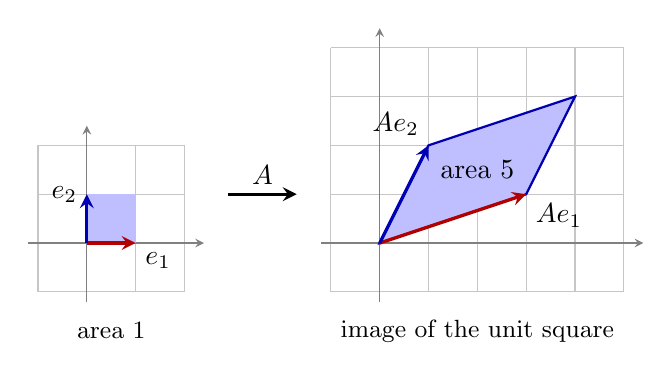
\begin{tikzpicture}[x=0.62cm,y=0.62cm,>=stealth]
  \draw[gray!45] (-1,-1) grid[step=1] (2,2);
  \draw[->,gray] (-1.2,0)--(2.4,0);
  \draw[->,gray] (0,-1.2)--(0,2.4);
  \fill[blue!25] (0,0) rectangle (1,1);
  \draw[->,very thick,red!70!black] (0,0)--(1,0);
  \draw[->,very thick,blue!70!black] (0,0)--(0,1);
  \node[below right] at (1,0) {$e_1$};
  \node[left] at (0,1) {$e_2$};
  \node at (0.5,-1.8) {\small area 1};
  \draw[->,very thick] (2.9,1)--(4.3,1);
  \node[above] at (3.6,1) {$A$};
  \begin{scope}[shift={(6,0)}]
    \draw[gray!45] (-1,-1) grid[step=1] (5,4);
    \draw[->,gray] (-1.2,0)--(5.4,0);
    \draw[->,gray] (0,-1.2)--(0,4.4);
    \fill[blue!25] (0,0)--(3,1)--(4,3)--(1,2)--cycle;
    \draw[thick,blue!70!black] (0,0)--(3,1)--(4,3)--(1,2)--cycle;
    \draw[->,very thick,red!70!black] (0,0)--(3,1);
    \draw[->,very thick,blue!70!black] (0,0)--(1,2);
    \node[below right] at (3,1) {$Ae_1$};
    \node[above left] at (1,2) {$Ae_2$};
    \node at (2,1.5) {area 5};
    \node at (2,-1.8) {\small image of the unit square};
  \end{scope}
\end{tikzpicture}
\end{center}

\textbf{Figure.} The matrix $A=\begin{bmatrix}3&1\\1&2\end{bmatrix}$ carries the unit square (area $1$) onto the parallelogram with vertices $(0,0)$, $(3,1)$, $(4,3)$ and $(1,2)$. Its area is $|\det A|=|3\cdot2-1\cdot1|=5$.

\begin{center}
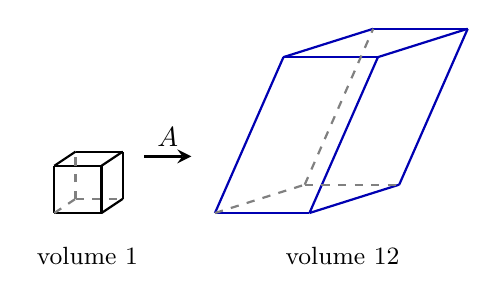
\begin{tikzpicture}[x=0.6cm,y=0.6cm,>=stealth]
  % cube spanned by e1, e2, e3
  \draw[thick] (0,0)--(1,0);
  \draw[thick] (0,0)--(0,1);
  \draw[thick] (0,1)--(1,1);
  \draw[thick] (0,1)--(0.45,1.3);
  \draw[thick] (0.45,1.3)--(1.45,1.3);
  \draw[thick] (1,0)--(1.45,0.3);
  \draw[thick] (1,0)--(1,1);
  \draw[thick] (1,1)--(1.45,1.3);
  \draw[thick] (1.45,0.3)--(1.45,1.3);
  \draw[thick,dashed,gray] (0,0)--(0.45,0.3);
  \draw[thick,dashed,gray] (0.45,0.3)--(1.45,0.3);
  \draw[thick,dashed,gray] (0.45,0.3)--(0.45,1.3);
  \node at (0.7,-0.9) {\small volume 1};
  \draw[->,very thick] (1.9,1.2)--(2.9,1.2);
  \node[above] at (2.4,1.2) {$A$};
  \begin{scope}[shift={(3.4,0)}]
    % parallelepiped spanned by (2,0,0), (1,2,0), (1,1,3)
    \draw[thick,blue!70!black] (0,0)--(2,0);
    \draw[thick,blue!70!black] (0,0)--(1.45,3.3);
    \draw[thick,blue!70!black] (1.45,3.3)--(3.45,3.3);
    \draw[thick,blue!70!black] (1.45,3.3)--(3.35,3.9);
    \draw[thick,blue!70!black] (3.35,3.9)--(5.35,3.9);
    \draw[thick,blue!70!black] (2,0)--(3.9,0.6);
    \draw[thick,blue!70!black] (2,0)--(3.45,3.3);
    \draw[thick,blue!70!black] (3.45,3.3)--(5.35,3.9);
    \draw[thick,blue!70!black] (3.9,0.6)--(5.35,3.9);
    \draw[thick,dashed,gray] (0,0)--(1.9,0.6);
    \draw[thick,dashed,gray] (1.9,0.6)--(3.9,0.6);
    \draw[thick,dashed,gray] (1.9,0.6)--(3.35,3.9);
    \node at (2.7,-0.9) {\small volume 12};
  \end{scope}
\end{tikzpicture}
\end{center}

\textbf{Figure.} The matrix $A=\begin{bmatrix}2&1&1\\0&2&1\\0&0&3\end{bmatrix}$ carries the unit cube (volume $1$, edges $e_1,e_2,e_3$) onto the parallelepiped with edges $Ae_1=(2,0,0)$, $Ae_2=(1,2,0)$ and $Ae_3=(1,1,3)$ (a perspective drawing; dashed edges are hidden behind the solid ones). Its volume is $|\det A|=2\cdot2\cdot3=12$, which is also the area $4$ of the base spanned by $Ae_1$ and $Ae_2$ times the height $3$.

\begin{think}{The determinant as a scale factor}{area}
(a)~For $A=\begin{bmatrix}3&1\\1&2\end{bmatrix}$ the unit square goes to a parallelogram of area $5$. What is the area of the image of the square with vertices $(0,0),(2,0),(2,2),(0,2)$? (b)~Each elementary matrix changes areas of the plane by a factor: a replacement $\begin{bmatrix}1&1\\0&1\end{bmatrix}$ is a shear, an interchange is a reflection in the line $x_1=x_2$, and $\begin{bmatrix}k&0\\0&1\end{bmatrix}$ stretches one direction. Find the factor for each, and compare it with $|\det E|$ (Theorem~\ref{thm:elementary}). (c)~Use (b) and the product rule to explain why every invertible $2\times2$ matrix multiplies areas by $|\det A|$. What happens for a singular matrix? (d)~In the second figure, why is the volume the base area times the height, and why is it equal to $|\det A|$? (e)~What information does the sign of $\det A$ carry that $|\det A|$ throws away? Think of the interchange.
\end{think}

\begin{think}{Scale factors multiply}{scale}
In the plane, $A$ multiplies areas by $5$ and $B$ by $3$. (a)~By what factor does the composite $AB$ multiply areas, and how does that relate to Theorem~\ref{thm:product}? (b)~By what factor does $A^{-1}$ multiply areas? (c)~Why can you not say by what factor $A+B$ multiplies areas?
\end{think}

\subsection*{Summary}
\begin{itemize}
  \item \textbf{Row operations.} Replacement leaves $\det$ unchanged; interchange reverses its sign; scaling a row by $k$ multiplies it by $k$. Two proportional rows, or a zero row, give $\det A=0$.
  \item \textbf{Computing.} Reduce to an echelon form $U$ with replacements and $r$ interchanges: $\det A=(-1)^r\times$ (product of the diagonal of $U$). Compare with cofactors in small examples.
  \item \textbf{Invertibility.} $A$ is invertible if and only if $\det A\neq0$: one more statement of the Invertible Matrix Theorem.
  \item \textbf{Products.} $\det(AB)=\det A\det B$, hence $\det A^{-1}=1/\det A$, $\det A^k=(\det A)^k$ and $\det AB=\det BA$. \textbf{Not} true: $\det(A+B)=\det A+\det B$, or $\det(rA)=r\det A$ (it is $r^n\det A$).
  \item \textbf{Transpose and columns.} $\det A\T=\det A$, so column operations act exactly as row operations.
  \item \textbf{Geometry.} $|\det A|$ is the factor by which $A$ multiplies areas (in the plane) and volumes (in space).
\end{itemize}

\subsection*{Questions to think about before the next section}
\begin{enumerate}
  \item The inverse of $\begin{bmatrix}a&b\\c&d\end{bmatrix}$ is $\dfrac1{ad-bc}\begin{bmatrix}d&-b\\-c&a\end{bmatrix}$. Is there a similar formula for $3\times3$ matrices that uses cofactors? Try to guess it from the $2\times2$ case, in which the cofactors of $a,b,c,d$ are $d,-c,-b,a$.
  \item For $\begin{bmatrix}a&b\\c&d\end{bmatrix}\bv{x}=\bv{y}$ with $ad-bc\neq0$, solve for $x_1$ by using the inverse. Write the numerator and the denominator as determinants. Does the pattern suggest what happens with three unknowns?
  \item Since $|\det A|$ is the factor by which $A$ multiplies areas, what does the number tell us about the image of a region that is not a square?
\end{enumerate}

\subsection*{Answers and discussion}
\begin{description}[leftmargin=0pt,itemsep=5pt]
  \item[Knowledge Check \ref{kc:effects}.] (a)~$7$ (replacement). (b)~$-7$ (interchange). (c)~$35$. (d)~Scaling by $\tfrac17$ gives $1$; the interchange then gives $-1$. (e)~Each of the three rows is multiplied by $2$: $2^3\cdot7=56$.
  \item[Knowledge Check \ref{kc:reduce}.] \begin{align*}
  \begin{bmatrix}1&3&2\\2&6&5\\-1&-2&3\end{bmatrix}
  &\rops{R_2-2R_1,\ R_3+R_1}
  \begin{bmatrix}1&3&2\\0&0&1\\0&1&5\end{bmatrix}
  \rops{R_2\leftrightarrow R_3}
  \begin{bmatrix}1&3&2\\0&1&5\\0&0&1\end{bmatrix}.
  \end{align*}
  One interchange, so the sign is $-$, and $\det=-(1\cdot1\cdot1)=-1$.
  \item[Knowledge Check \ref{kc:param}.] Expanding along row $1$: $h\begin{vmatrix}h&1\\2&h\end{vmatrix}-2\begin{vmatrix}1&1\\0&h\end{vmatrix}=h(h^2-2)-2h=h^3-4h=h(h-2)(h+2)$. The matrix is not invertible for $h=0,\,2,\,-2$.
  \item[Knowledge Check \ref{kc:product}.] (a)~$(-2)(5)=-10$. (b)~$-2$. (c)~$-\tfrac12$. (d)~$(-2)^2/5=\tfrac45$. You can also find $\det(3A)=3^3(-2)=-54$ and $\det(-B)=(-1)^3\cdot5=-5$ (Theorem~\ref{thm:scalar}). You cannot find $\det(A+B)$: there is no rule, and different matrices with the same determinants give different answers.
  \item[Knowledge Check \ref{kc:truefalse}.] (a)~False (Sum trap). (b)~False: $\det(2A)=8\det A$. (c)~True (Theorem~\ref{thm:inverse}). (d)~False: it is $1/\det A$. (e)~True: $\det(A\T B)=\det A\T\det B=\det A\det B$.
  \item[Knowledge Check \ref{kc:zero}.] (a)~Row $2$ is $2\times$ row $1$ (Theorem~\ref{thm:equalrows}). (b)~Column $2$ is zero (Theorem~\ref{3.1-thm:zero}). (c)~Column $3$ is the sum of columns $1$ and $2$: the column operation $C_3-C_1-C_2$ does not change the determinant and creates a zero column.
  \item[Pause and think \ref{think:swap}.] (a)~Interchanging two equal rows gives back the same matrix $A$, so $\det A=-\det A$, hence $2\det A=0$ and $\det A=0$. (b)~Multiply row $p$ by $\tfrac13$ (Theorem~\ref{thm:rowops}(c)): the new matrix has two equal rows, so its determinant is $0$ by part (a), and $0=\tfrac13\det A$ gives $\det A=0$. (c)~The base case $2\times2$: swapping two equal rows reverses the sign while leaving the matrix unchanged. In the earlier Pause and think the alternating signs $+,-$ made exactly this cancellation work, $ab-ba=0$.
  \item[Pause and think \ref{think:cost}.] (a)~$\tfrac23\cdot25^3=\tfrac23\cdot15625\approx10{,}417$ operations, against $1.55\times10^{25}$: elimination is faster by a factor of about $10^{21}$. At $10^{12}$ operations per second it takes about $10^{-8}$ s. (b)~$(2n)^3=8n^3$: the work grows by a factor $8$. (c)~The determinant of a triangular matrix is the product of the diagonal entries, whatever they are. The reduced echelon form asks for pivots equal to $1$, which needs a scaling of every row, and a scaling changes the determinant and must be tracked.
  \item[Pause and think \ref{think:squares}.] (a)~$(\det A)^2=\det(A^2)=\det I=1$, so $\det A=\pm1$. Both occur: $I$ has determinant $1$ and $\begin{bmatrix}0&1\\1&0\end{bmatrix}$ (an interchange) has determinant $-1$. (b)~$(\det A)^3=0$, so $\det A=0$. (c)~$(\det A)^2=\det A$, so $\det A\in\{0,1\}$; $I$ and $\mathbf{0}$ show both occur. If $A$ is invertible, multiply $A^2=A$ by $A^{-1}$ to get $A=I$.
  \item[Pause and think \ref{think:rowlinear}.] (a)~$(a+a')d-(b+b')c=(ad-bc)+(a'd-b'c)$. (b)~$\begin{vmatrix}1&2\\3&4\end{vmatrix}=-2$, and $\begin{vmatrix}1&0\\3&4\end{vmatrix}+\begin{vmatrix}0&2\\3&4\end{vmatrix}=4+(-6)=-2$. (c)~The rule needs the other row to stay the same: only \emph{one} row is split. In $A+B$ every row changes at once (and, as the example $\operatorname{diag}(1,0)+\operatorname{diag}(0,1)$ shows, the determinant of the sum has no connection with the determinants of the parts).
  \item[Pause and think \ref{think:oddskew}.] (a)~$\det A=\det A\T=\det(-A)=(-1)^n\det A=-\det A$ for $n$ odd. Hence $2\det A=0$ and $\det A=0$. (b)~For even $n$ the factor $(-1)^n=+1$ gives no information. The matrix $\begin{bmatrix}0&a\\-a&0\end{bmatrix}$ has determinant $a^2$, which is not zero for $a\neq0$.
  \item[Pause and think \ref{think:area}.] (a)~The square of side $2$ is the unit square scaled by $2$ and $A$ is linear, so its image is the first parallelogram scaled by $2$ in every direction; the area is $4\cdot5=20$. (b)~The shear $\begin{bmatrix}1&1\\0&1\end{bmatrix}$ slides each horizontal line sideways and keeps its base and height, so area is unchanged: factor $1=|\det E|$. The reflection keeps all lengths: factor $1=|-1|$. The stretch multiplies area by $|k|=|\det E|$. (c)~Every invertible $A$ is a product $F_1\cdots F_p$ of elementary matrices, each of which multiplies areas by $|\det F_i|$, so $A$ multiplies areas by $|\det F_1|\cdots|\det F_p|=|\det A|$ (product rule). A singular $A$ squeezes the plane into a line or a point, so the area is $0=|\det A|$. (d)~The base is the parallelogram spanned by $Ae_1=(2,0,0)$ and $Ae_2=(1,2,0)$ in the floor plane, with area $|2\cdot2-0\cdot1|=4$, and $Ae_3=(1,1,3)$ rises $3$ units above the floor. Volume is the product $4\cdot3=12$, and since $A$ is triangular, $\det A=2\cdot2\cdot3=12$. (e)~The sign records whether $A$ reverses orientation (as an interchange does) or preserves it. The area ignores that.
  \item[Pause and think \ref{think:scale}.] (a)~$5\cdot3=15$. The composite scales areas by $|\det A|\,|\det B|=|\det AB|$, which is Theorem~\ref{thm:product} seen geometrically. (b)~$\tfrac15$, as in Theorem~\ref{thm:inverse}(a). (c)~There is no connection between the determinants of $A$, $B$ and of $A+B$ (Sum trap). The scale factors of a sum depend on the matrices themselves.
  \item[Before the next section.] (1)~For $2\times2$ the entries of the inverse are the cofactors divided by $\det A$, in transposed positions (the cofactor of $b$ is $-c$ and it sits in the position of $c$). A natural guess for $3\times3$ is the transposed matrix of cofactors divided by $\det A$; it can be tested on a triangular example. (2)~From $\bv{x}=A^{-1}\bv{y}$: $x_1=\dfrac{dy_1-by_2}{ad-bc}=\dfrac{\begin{vmatrix}y_1&b\\y_2&d\end{vmatrix}}{\begin{vmatrix}a&b\\c&d\end{vmatrix}}$. The numerator is the determinant of the matrix with its first column replaced by $\bv{y}$. The same pattern is expected for three unknowns. (3)~The same factor applies to the area of any region, since a region can be filled by small squares, each of which is multiplied by $|\det A|$.
\end{description}

\end{document}
